\bibliography{references}

%\apendices
%
%\chapter{Artigo Científico}
%\label{chap:apendice}
%
%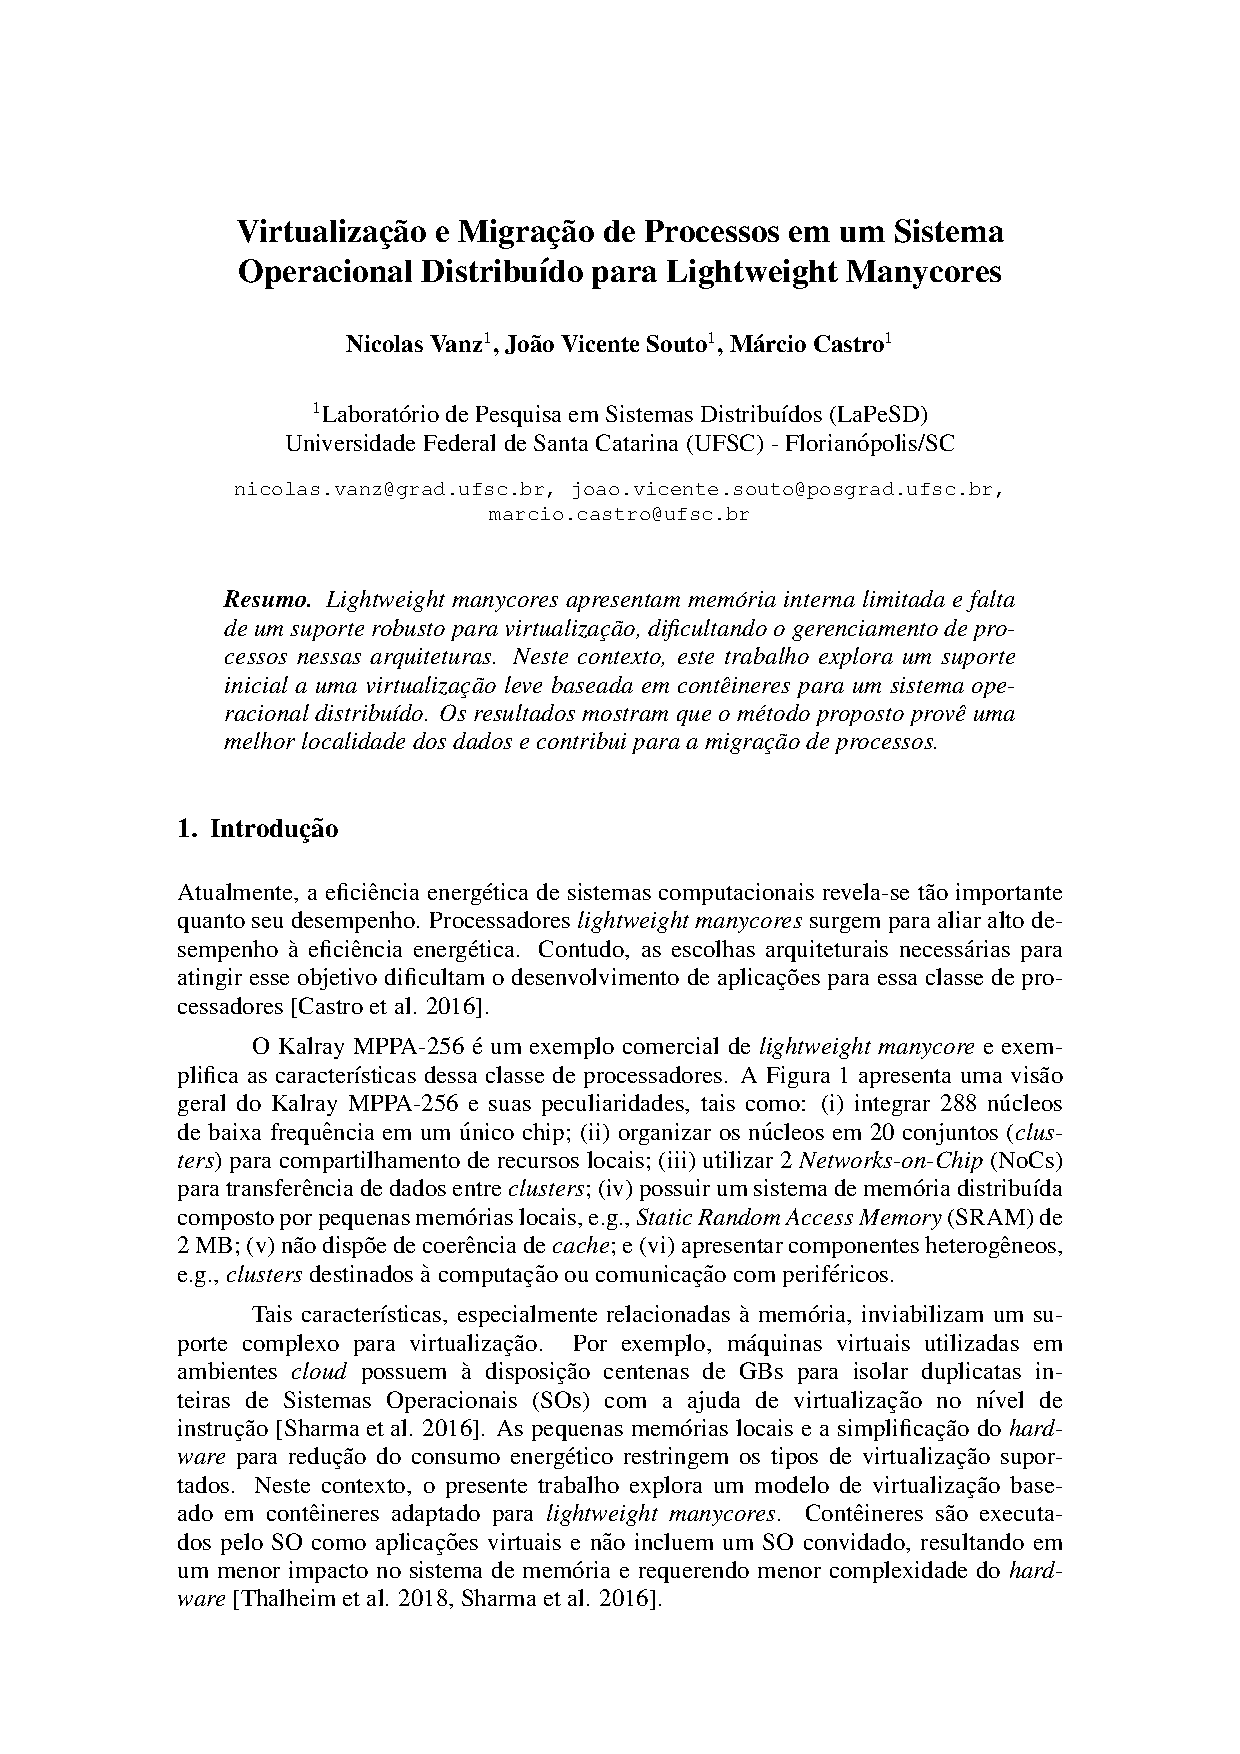
\includepdf[scale=1,pages=-,pagecommand={}]{content/apendices/erad.pdf}

% Uso de \cite em apêndice/anexo como se fossem antes do \bibliography{}.  NBR
% 14724 e NBR 6023, assim como os documentos da BU não especificam nada sobre
% citações dentro de apêndices/anexos. No entanto, em email trocado com a BU, a
% orientação foi de usar \cite{} normalmente e deixar que as referências sejam
% listadas na única bibliografia do documento, mesmo que esta esteja antes dos
% apêndices. A argumentação é que apêndices e anexos são numerados e fazem parte
% do documento, logo suas referências devem ser listadas como referências do
% documento. Além disso as normas não prevem segmentar as referências por
% capítulos.
